\documentclass[11pt, a4paper]{article}
\usepackage[utf8]{inputenc}
\usepackage{amsmath, amssymb, amsfonts}
\usepackage{geometry}
\usepackage{graphicx}
\usepackage{tikz}
\usepackage{hyperref}
\usepackage{booktabs}
\usepackage{float}

% --- TikZ Setup for Diagrams ---
\usetikzlibrary{shapes, arrows, positioning, calc, fit, backgrounds, shadows, decorations.pathreplacing}

\tikzset{
    block/.style = {rectangle, draw, fill=blue!5, text centered, rounded corners, minimum height=3em, minimum width=3cm},
    process/.style = {rectangle, draw, fill=green!5, text centered, rounded corners, minimum height=3em},
    decision/.style = {diamond, draw, fill=red!5, text centered, aspect=2},
    line/.style = {draw, -latex', thick},
    dashedline/.style = {draw, -latex', dashed, thick},
    container/.style = {draw, rectangle, dashed, inner sep=1em, fill=gray!5}
}
% -------------------------------

\geometry{margin=1in}

\title{\textbf{Implementation Report: Physics-Informed Variational Autoencoder (PIVAE) for Airfoil Parameterization}}
\author{Robert Flassig}
\date{\today}

\begin{document}

\maketitle

\section{Introduction}
This report documents the implementation of a Physics-Informed Variational Autoencoder (PIVAE) designed for the generative design and analysis of airfoil geometries. The architecture adopts the airfoil generator (AG) methodology proposed by \emph{Kang et al. (2025)}, which addresses the limitations of traditional generative models regarding feasibility and intuitiveness. The system utilizes a split-network architecture to decouple thickness and camber distributions, ensuring topological validity (non-intersection) and providing direct control over aerodynamic features.

\section{Methodology Overview}

The overall approach treats airfoil parameterization as a dimensionality reduction problem where high-dimensional coordinates are compressed into a low-dimensional, physically interpretable latent space.

\begin{figure}[H]
    \centering
    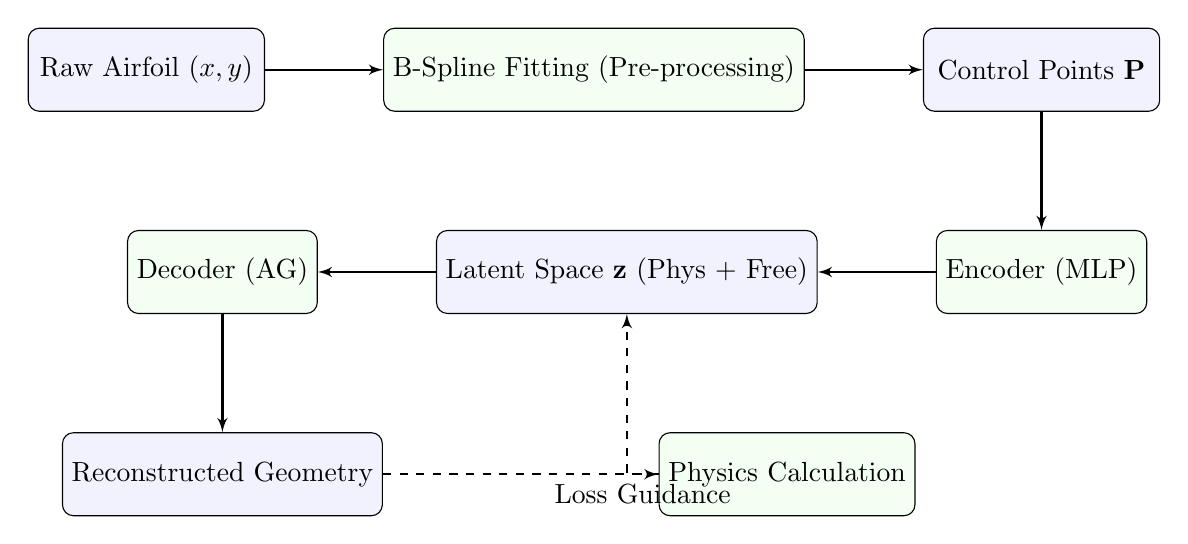
\begin{tikzpicture}[node distance=1.5cm, auto]
        % Nodes
        \node [block] (input) {Raw Airfoil $(x,y)$};
        \node [process, right=of input] (fitting) {B-Spline Fitting (Pre-processing)};
        \node [block, right=of fitting] (cps) {Control Points $\mathbf{P}$};
        \node [process, below=of cps] (encoder) {Encoder (MLP)};
        \node [block, left=of encoder] (latent) {Latent Space $\mathbf{z}$ (Phys + Free)};
        \node [process, left=of latent] (decoder) {Decoder (AG)};
        \node [block, below=of decoder] (recon) {Reconstructed Geometry};
        
        % Edges
        \path [line] (input) -- (fitting);
        \path [line] (fitting) -- (cps);
        \path [line] (cps) -- (encoder);
        \path [line] (encoder) -- (latent);
        \path [line] (latent) -- (decoder);
        \path [line] (decoder) -- (recon);
        
        % Physics Feedback
        \node [process, right=of recon, xshift=2cm] (physics) {Physics Calculation};
        \path [dashedline] (recon) -- (physics);
        \path [dashedline] (physics) -| node[near start, below] {Loss Guidance} (latent);
    \end{tikzpicture}
    \caption{Overview of the PIVAE approach. Raw data is converted to control points using a clustered topology, encoded into a disentangled latent space, and reconstructed via a physics-constrained decoder.}
    \label{fig:overview}
\end{figure}

One core innovation of this PIVAE is the dual-alignment strategy that bridges the gap between the Encoder's latent space and the Decoder's physical output.

\begin{figure}[H]
    \centering
    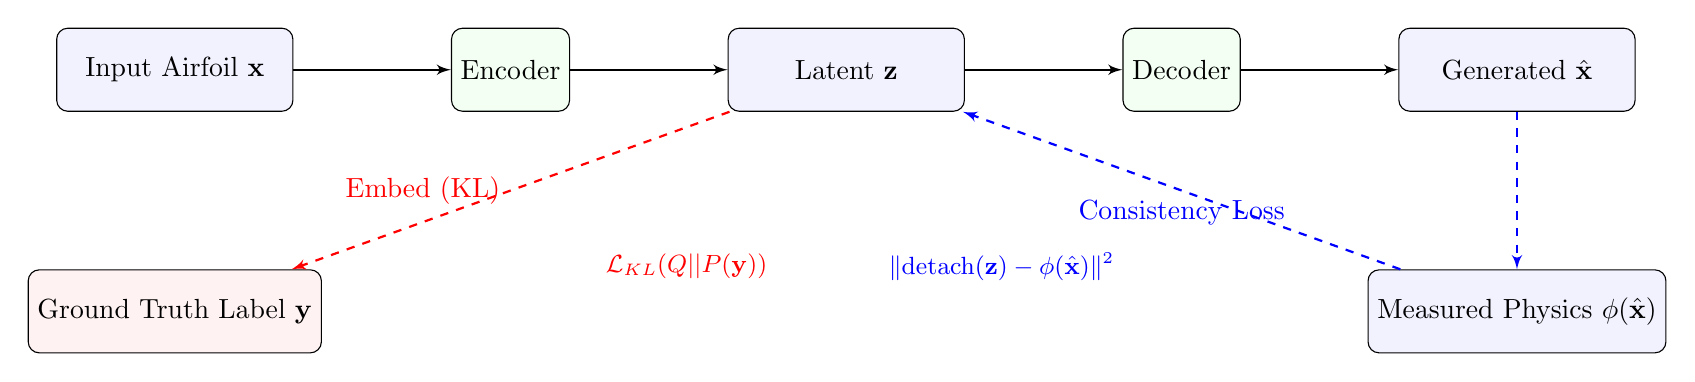
\begin{tikzpicture}[node distance=1.5cm, auto]
        % Main Flow
        \node [block] (input) {Input Airfoil $\mathbf{x}$};
        \node [process, right=2cm of input] (encoder) {Encoder};
        \node [block, right=2cm of encoder] (latent) {Latent $\mathbf{z}$};
        \node [process, right=2cm of latent] (decoder) {Decoder};
        \node [block, right=2cm of decoder] (output) {Generated $\hat{\mathbf{x}}$};
        
        % Edges Main
        \path [line] (input) -- (encoder);
        \path [line] (encoder) -- (latent);
        \path [line] (latent) -- (decoder);
        \path [line] (decoder) -- (output);
        
        % Labels & Measures
        \node [block, below=2cm of input, fill=red!5] (label) {Ground Truth Label $\mathbf{y}$};
        \node [block, below=2cm of output, fill=blue!5] (measure) {Measured Physics $\phi(\hat{\mathbf{x}})$};
        
        % Loss Arrows
        \draw [dashedline, red] (latent) -- node[midway, left] {Embed (KL)} (label);
        \path [dashedline, blue] (output) -- (measure);
        \path [dashedline, blue] (measure) -- node[midway, below] {Consistency Loss} (latent);
        
        % Gradient Stop Notation
        \node [text=red, font=\small, align=center] at (6.5, -2.5) {$\mathcal{L}_{KL}(Q || P(\mathbf{y}))$};
        \node [text=blue, font=\small, align=center] at (10.5, -2.5) {$\|\text{detach}(\mathbf{z}) - \phi(\hat{\mathbf{x}})\|^2$};

    \end{tikzpicture}
    \caption{The "Bridge" Strategy. The latent space is anchored from two sides: (1) The Encoder is forced to place latents at the correct physical label coordinates via KL divergence. (2) The Decoder is forced to respect these latents via a Consistency Loss that measures the generated geometry.}
    \label{fig:bridge}
\end{figure}

\section{Geometric Parameterization}

\subsection{Decomposition and B-Spline Representation}
To guarantee geometric feasibility, the airfoil is not represented as a single coordinate loop but is decomposed into two independent curves defined over the normalized chord $x \in [0, 1]$:
\begin{enumerate}
    \item \textbf{Thickness Distribution ($T(x)$):} Symmetric thickness added to the mean line.
    \item \textbf{Camber Distribution ($C(x)$):} The curvature of the mean line.
\end{enumerate}
The physical upper ($y_u$) and lower ($y_l$) surfaces are derived as:
\begin{equation}
    y_u(x) = C(x) + \frac{1}{2}T(x), \quad y_l(x) = C(x) - \frac{1}{2}T(x)
\end{equation}

\subsection{Clustered Knot Vector Topology}
Standard uniform B-splines often struggle to capture the high curvature gradients at the Leading Edge (LE), leading to "sharp nose" artifacts. To resolve this, we employ a \textbf{Clustered Knot Vector} where the knot density follows a power law ($t \sim x^2$):
\begin{equation}
    \text{Knots} = \{0, 0, 0, 0, 0.01, 0.04, 0.09, \dots, 1, 1, 1, 1\}
\end{equation}
This allocates a higher density of control points ($P_0, P_1, P_2$) to the first 5\% of the chord, providing the necessary resolution to model a perfectly round LE radius without increasing the total number of parameters ($N=16$).

\begin{figure}[H]
    \centering
    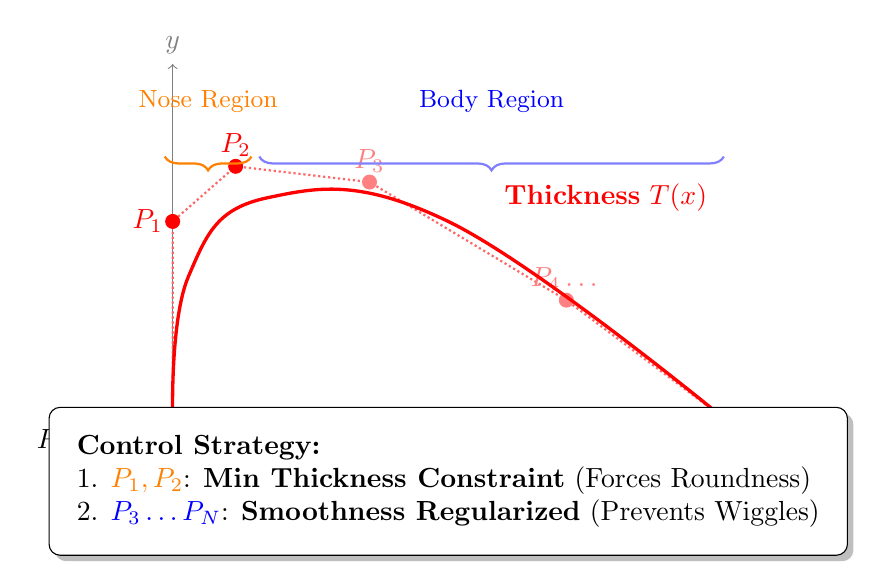
\begin{tikzpicture}[scale=1.0]
        % Axes
        \draw[->, gray] (-0.5,0) -- (7.5,0) node[right] {$x$};
        \draw[->, gray] (0,-1.0) -- (0,4.5) node[above] {$y$};

        % --- COORDINATES ---
        \coordinate (P0) at (0,0);
        \coordinate (P1) at (0, 2.5);   % Vertical constraint P1
        \coordinate (P2) at (0.8, 3.2); % P2
        \coordinate (P3) at (2.5, 3.0); % P3
        \coordinate (P4) at (5.0, 1.5); % P4
        \coordinate (End) at (7.0, 0);

        % --- CONTROL POLYGON ---
        \draw[red!60, thick, densely dotted] (P0) -- (P1) -- (P2) -- (P3) -- (P4) -- (End);
        
        % --- POINTS (Clustered Visual) ---
        \filldraw [black] (P0) circle (2.5pt) node[below left] {$P_0 (Fixed)$};
        \filldraw [red] (P1) circle (2.5pt) node[left] {$P_1$};
        \filldraw [red] (P2) circle (2.5pt) node[above] {$P_2$};
        \filldraw [red!50] (P3) circle (2.5pt) node[above] {$P_3$};
        \filldraw [red!50] (P4) circle (2.5pt) node[above] {$P_4 \dots$};
        
        % --- CURVE (Smooth) ---
        \draw [red, very thick] plot [smooth, tension=0.7] coordinates { (0,0) (0.2, 1.8) (1.2, 2.8) (3.5, 2.5) (7.0, 0) };
        \node[red] at (5.5, 2.8) {\textbf{Thickness} $T(x)$};

        % --- ZONES ---
        % Nose Zone
        \draw[thick, orange, decorate, decoration={brace,amplitude=5pt,raise=5pt}] (1.0, 3.5) -- (-0.1, 3.5) node[midway, yshift=15pt, text=orange, font=\small] {Nose Region};
        
        % Body Zone
        \draw[thick, blue!50, decorate, decoration={brace,amplitude=5pt,raise=5pt}] (7.0, 3.5) -- (1.1, 3.5) node[midway, yshift=15pt, text=blue, font=\small] {Body Region};

        % --- ANNOTATION BOX ---
        \node [draw, fill=white, drop shadow, rounded corners, align=left, inner sep=10pt] at (3.5, -0.8) {
            \textbf{Control Strategy:}\\
            1. \textcolor{orange}{$P_1, P_2$}: \textbf{Min Thickness Constraint} (Forces Roundness)\\
            2. \textcolor{blue}{$P_3 \dots P_N$}: \textbf{Smoothness Regularized} (Prevents Wiggles)
        };

    \end{tikzpicture}
    \caption{Clustered Control Point Parameterization. Points $P_1$ and $P_2$ are packed near the leading edge to control the nose radius. The loss function treats these zones differently to avoid conflicting objectives.}
    \label{fig:cp_placement}
\end{figure}

\subsection{Preprocessing: Constrained Fitting}
We convert raw coordinate data into control points using a constrained least squares algorithm that respects the $P_0=(0,0)$ constraint while leveraging the clustered basis matrix $\mathbf{M}_{clust}$:
\begin{equation}
    \min_{\mathbf{P}_{free}} \| \mathbf{M}_{clust} \mathbf{P} - \mathbf{Y}_{target} \|^2 + \lambda \| \mathbf{D}^2 \mathbf{P} \|^2
\end{equation}

\section{Decoder Process Scheme}

The decoder translates the latent vector $\mathbf{z}$ back into control points. To ensure physical validity (e.g., non-negative thickness and a round nose), we apply region-specific activation functions.

\begin{figure}[H]
    \centering
    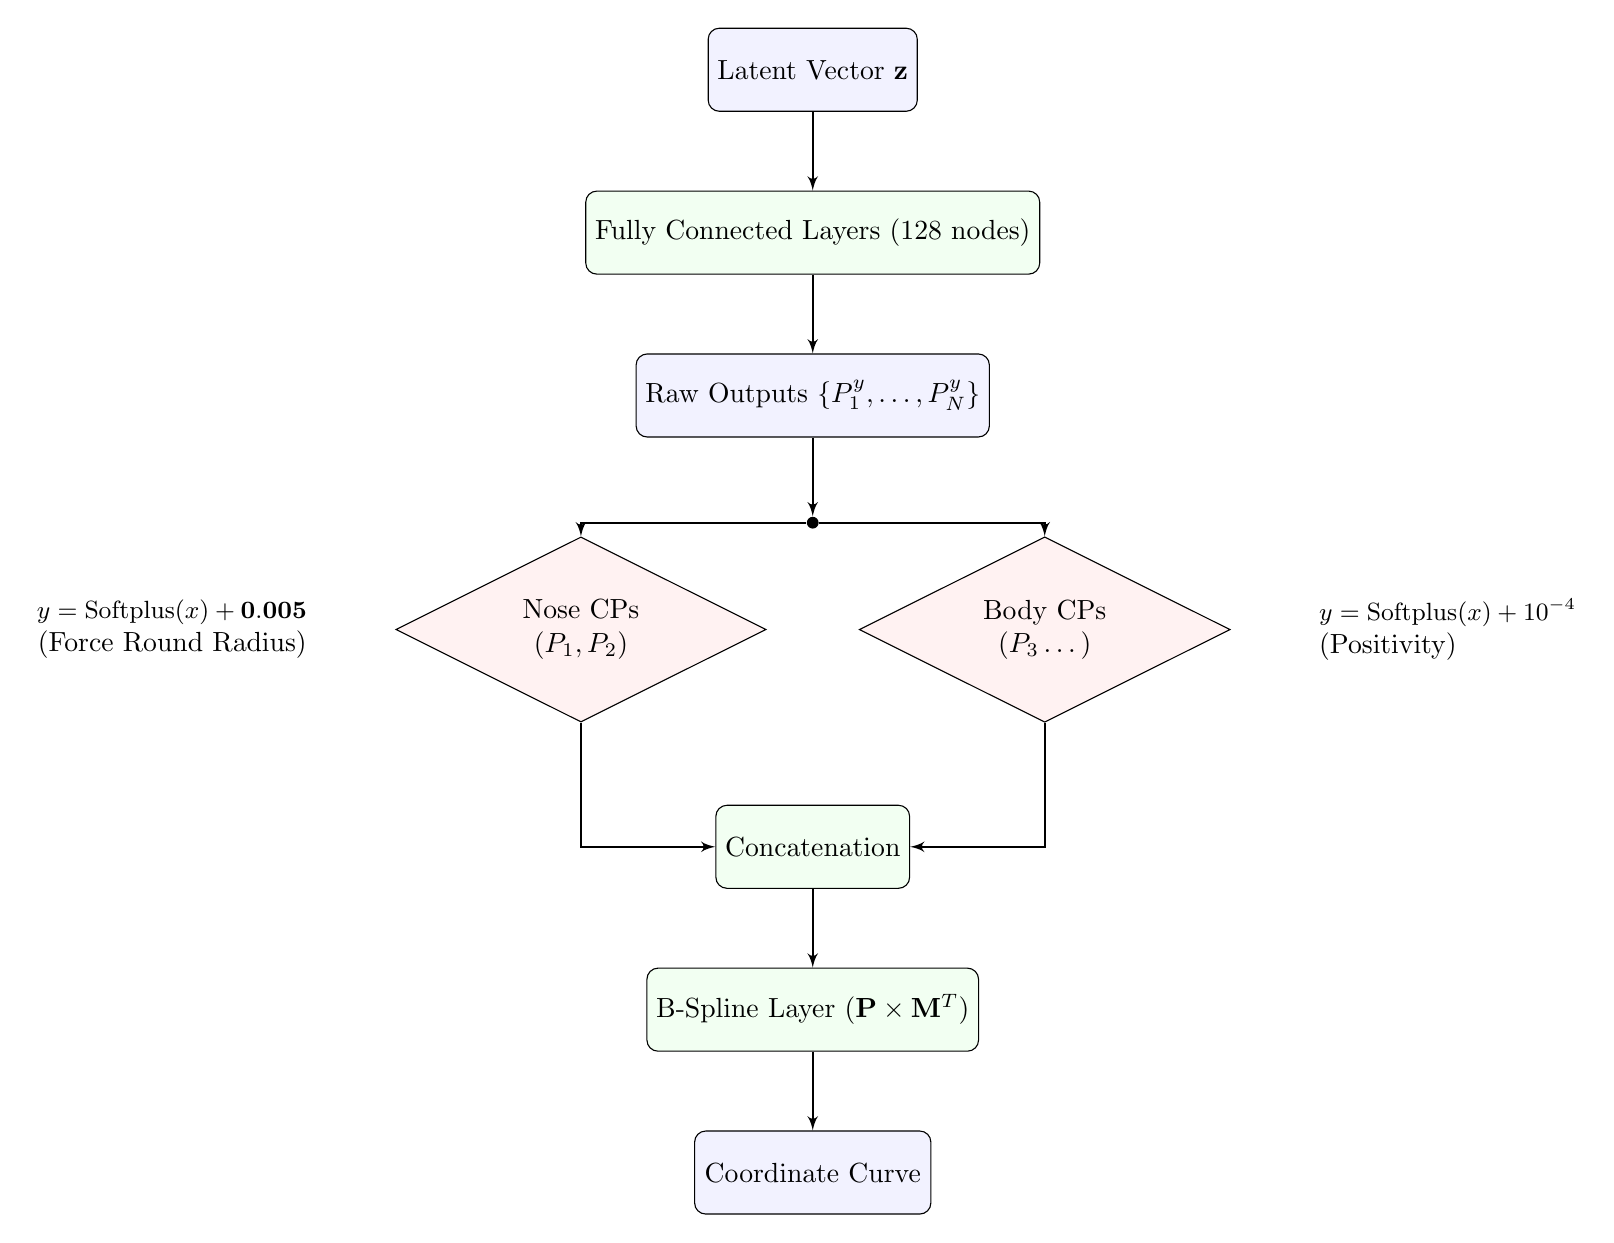
\begin{tikzpicture}[node distance=1.0cm, auto]
        % Latent Input
        \node [block, minimum width=2cm] (z) {Latent Vector $\mathbf{z}$};
        
        % MLP Layers
        \node [process, below=of z] (mlp) {Fully Connected Layers (128 nodes)};
        
        % Raw Output
        \node [block, below=of mlp] (raw) {Raw Outputs $\{P_1^y, \dots, P_N^y\}$};
        
        % Split
        \node (split) [below=of raw, circle, fill=black, inner sep=1.5pt] {};
        
        % Nose Constraint
        \node [decision, below left=of split, xshift=-1cm, text width=2.5cm] (nose) {Nose CPs $(P_1, P_2)$};
        \node [left=of nose, align=right] {\small $y = \text{Softplus}(x) + \mathbf{0.005}$\\(Force Round Radius)};
        
        % Body Constraint
        \node [decision, below right=of split, xshift=1cm, text width=2.5cm] (body) {Body CPs $(P_3 \dots)$};
        \node [right=of body, align=left] {\small $y = \text{Softplus}(x) + 10^{-4}$\\(Positivity)};
        
        % Recombine
        \node [process, below=of split, yshift=-2.5cm] (concat) {Concatenation};
        
        % B-Spline
        \node [process, below=of concat] (bspline) {B-Spline Layer ($\mathbf{P} \times \mathbf{M}^T$)};
        
        % Output
        \node [block, below=of bspline] (output) {Coordinate Curve};
        
        % Arrows
        \path [line] (z) -- (mlp);
        \path [line] (mlp) -- (raw);
        \path [line] (raw) -- (split);
        \path [line] (split) -| (nose);
        \path [line] (split) -| (body);
        \path [line] (nose) |- (concat);
        \path [line] (body) |- (concat);
        \path [line] (concat) -- (bspline);
        \path [line] (bspline) -- (output);
        
    \end{tikzpicture}
    \caption{Decoder Scheme with Region-Specific Constraints. A higher bias is applied to the nose control points ($P_1, P_2$) to prevent the leading edge from collapsing into a sharp wedge.}
    \label{fig:decoder}
\end{figure}

\section{Physics Alignment and Training Strategy}

\subsection{Embedding Strategy}
The latent space $\mathbf{z} \in \mathbb{R}^{12}$ is split to disentangle physical properties from stylistic features.
\begin{itemize}
    \item \textbf{Physical Latents ($\mathbf{z}_{phys} \in \mathbb{R}^3$ per branch):} These dimensions are explicitly trained to track specific aerodynamic features (Max Thickness, Max Camber, LE Radius, TE Direction).
    \item \textbf{Free Latents ($\mathbf{z}_{free} \in \mathbb{R}^3$ per branch):} These dimensions are governed only by the reconstruction and KL terms, allowing them to capture residual geometric variations not described by standard parameters.
\end{itemize}

We employ a split latent space $\mathbf{z} \in \mathbb{R}^{12}$, divided into \textbf{Physical} ($\mathbf{z}_{phys}$) and \textbf{Free} ($\mathbf{z}_{free}$) variables.

\subsubsection{Physics-Informed Prior (Encoder Side)}
Instead of a standard Gaussian prior $\mathcal{N}(0, 1)$, the physical dimensions are trained against a dynamic prior centered on the ground truth labels:
\begin{equation}
    \mathcal{L}_{KL} = D_{KL}\left( q(\mathbf{z}|\mathbf{x}) \parallel \mathcal{N}(\mathbf{y}_{label}, \sigma_{prior}^2) \right)
\end{equation}
This explicitly forces the encoder to map the latent variable $z_0$ directly to the physical value (e.g., max thickness), while the learned prior variance $\sigma_{prior}^2$ allows the model to capture aleatoric uncertainty (handling Out-of-Distribution samples gracefully).

\subsubsection{Latent Consistency with Gradient Stop (Decoder Side)}
To prevent "Posterior Collapse" (where the decoder ignores the physics latent and outputs an average shape), we measure the physics of the \textit{generated} geometry $\phi(\hat{\mathbf{x}})$ and force it to match the latent mean.

\textbf{Crucial Implementation Detail:} We detach the latent mean from the computation graph for this term:
\begin{equation}
    \mathcal{L}_{consist} = \| \text{detach}(\mathbf{\mu}_{z}) - \phi(\text{Decode}(\mathbf{z})) \|^2
\end{equation}
This ensures that gradients flow \textbf{only} to the Decoder (forcing it to fix the shape) and not to the Encoder (preventing the Encoder from "cheating" by shifting the mean to match a bad reconstruction).

\subsection{Loss Function and Training}

The training objective minimizes a composite loss function comprising four key terms. To ensure stable convergence, we employ a **Normalized Weighting Strategy** where each term is scaled to the same order of magnitude ($O \approx 10^1$) before dynamic annealing is applied.

\begin{equation}
    \mathcal{L} = \lambda_{rec}\mathcal{L}_{rec} + \beta(\lambda_{kl}\mathcal{L}_{kl}) + \alpha(\lambda_{phys}\mathcal{L}_{consist}) + \lambda_{reg}\mathcal{L}_{reg}
\end{equation}

\subsubsection{Split \& Rebalanced Reconstruction ($\mathcal{L}_{rec}$)}
Standard MSE is dominated by thickness errors ($O(10^{-2})$), causing the network to ignore the much smaller camber errors ($O(10^{-4})$). To fix the "flat camber" issue, we split the reconstruction loss and amplify the camber term:
\begin{equation}
    \mathcal{L}_{rec} = \sum w_i (y_{thick} - \hat{y}_{thick})^2 + \mathbf{20.0} \times \sum w_i (y_{camber} - \hat{y}_{camber})^2
\end{equation}
where $w_i$ is the Kulfan weighting, amplifying leading edge errors ($x < 0.2$) by a factor of 20.0.

\subsubsection{Physics Embedding via KL Divergence ($\mathcal{L}_{kl}$)}
This term trains the \textbf{Encoder}. For the physical latent variables $\mathbf{z}_{phys}$, we replace the standard Gaussian prior with a physics-informed dynamic prior centered on the ground truth labels $\mathbf{y}$:
\begin{equation}
    \mathcal{L}_{kl\_phys} = D_{KL}\left( q(\mathbf{z}|\mathbf{x}) \parallel \mathcal{N}(\mathbf{y}, \sigma_{prior}^2) \right)
\end{equation}
This forces the encoder to map latent variables directly to physical quantities (e.g., $z_0 \to \text{Thickness}_{max}$), while the learnable prior variance $\sigma_{prior}^2$ allows the model to handle uncertainty. Free variables $\mathbf{z}_{free}$ are regularized against a standard $\mathcal{N}(0, I)$ prior.

\subsubsection{Latent Consistency with Gradient Stop ($\mathcal{L}_{consist}$)}
This term trains the \textbf{Decoder}. We measure the physical properties of the \textit{generated} geometry $\phi(\hat{\mathbf{x}})$ and force them to match the latent mean $\mu_z$. To prevent the encoder from "cheating" (shifting $\mu_z$ to match a bad reconstruction), we detach the target:
\begin{equation}
    \mathcal{L}_{consist} = \| \text{detach}(\mathbf{\mu}_{z}) - \phi(\text{Decode}(\mathbf{z})) \|^2
\end{equation}
This ensures gradients flow \textbf{only} to the decoder, forcing it to generate shapes that respect the latent control variables.

\subsubsection{Body-Only Smoothness ($\mathcal{L}_{reg}$)}
To allow for the high curvature required at the nose, smoothness regularization (second derivative penalty) is applied \textbf{only} to control points $P_3 \dots P_N$, explicitly ignoring the nose region ($P_0, P_1, P_2$).

\subsubsection{Scheduling Strategy}
\begin{itemize}
    \item \textbf{Cyclical Annealing ($\beta$):} The KL weight $\beta$ cycles linearly from $0.0 \to 1.0$ every 20 epochs. This periodic "breathing" prevents posterior collapse.
    \item \textbf{Delayed Physics Ramp ($\alpha$):} The physics consistency weight $\alpha$ is kept at 0.0 for the first 15 epochs ("Geometry First" phase). Once the geometry is stable, $\alpha$ is ramped to $1.0$ to enforce physical alignment.
\end{itemize}

\end{document}